\subsubsection{Idee}
\begin{frame}[fragile]{Idee}
\begin{columns}
\column{0.5\textwidth}
    \begin{alertblock}{Zeige Aussagen der Form:\\\emph{Für alle $n\in\mathbb{N}$ gilt...}}
    \begin{enumerate}
        \item Zeige Aussage für das kleinste Element
        \item<1-> \only<7,8|handout:0>{\alert<7>{Zeige, wenn Aussage für beliebiges $n$ gilt, gilt sie auch für dessen Nachfolger, also $n+1$.}}\onslide<1-6>{Zeige, dass Aussage auch für das folgende Element gilt.}
        \item<2-6,8> \only<8|handout:0>{\alert<8>{$\leadsto$ Aussage gilt für alle $n$.}}\onslide<2-6>{\small Zeige, dass Aussage auch für das folgende Element gilt.}
        \item<3-6> \footnotesize Zeige, dass Aussage auch für das folgende Element gilt.
        \item<4-6> \scriptsize Zeige, dass Aussage auch für das folgende Element gilt.
        \item<5-6> \tiny Zeige, dass Aussage auch für das folgende Element gilt.
        \item<6> \dots
    \end{enumerate}
    \end{alertblock}
\column{0.5\textwidth}
    \begin{figure}
        \centering
        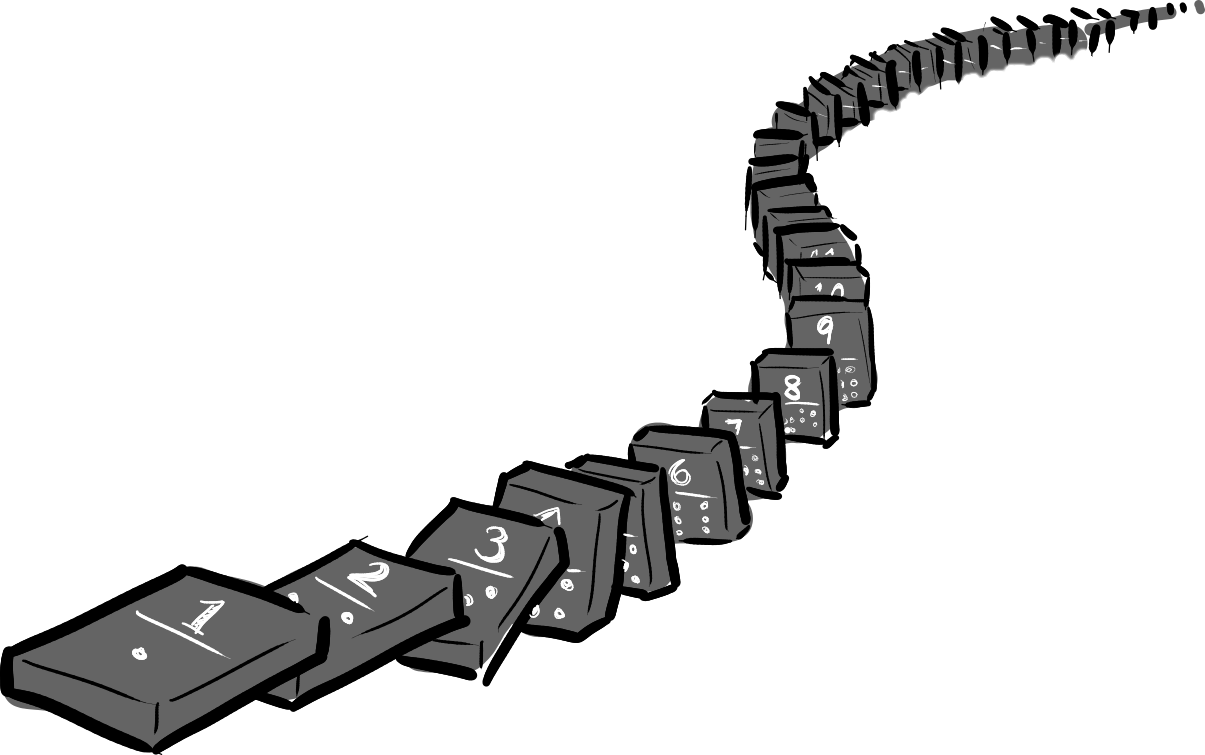
\includegraphics[width=0.7\textwidth]{../figures/induction.png}
        %\caption{Idee}
        %
    \end{figure}
\end{columns}
\end{frame}

\subsubsection{Funktionsweise}
\begin{frame}[fragile]{Struktur}
    \begin{alertblock}{Zeige Aussagen der Form:\\\emph{Für alle $n\in\mathbb{N}$ gilt...}}
    \begin{enumerate}
        \item \alert{Induktionsanfang}\\Zeige Aussage für das kleinste Element
        \item \alert{Induktionsvorraussetzung}\\Zeige, unter der Vorraussetzung: \\\emph{die Aussage gelte für beliebiges $n$},\dots
        \item \alert{Induktionsschritt}\\\dots dann gilt die Aussage auch für dessen Nachfolger $n+1$.
        \item $\leadsto$ Aussage gilt für alle $n \in \mathbb{N}$.
    \end{enumerate}
    \end{alertblock}
\end{frame}

\begin{frame}[fragile]{Beispiel}
\center $\displaystyle\sum_{i = 0}^{n} (2i+1) = (n+1)^2,\quad\forall n \in\mathbb{N}$.
    \begin{figure}
        \centering
        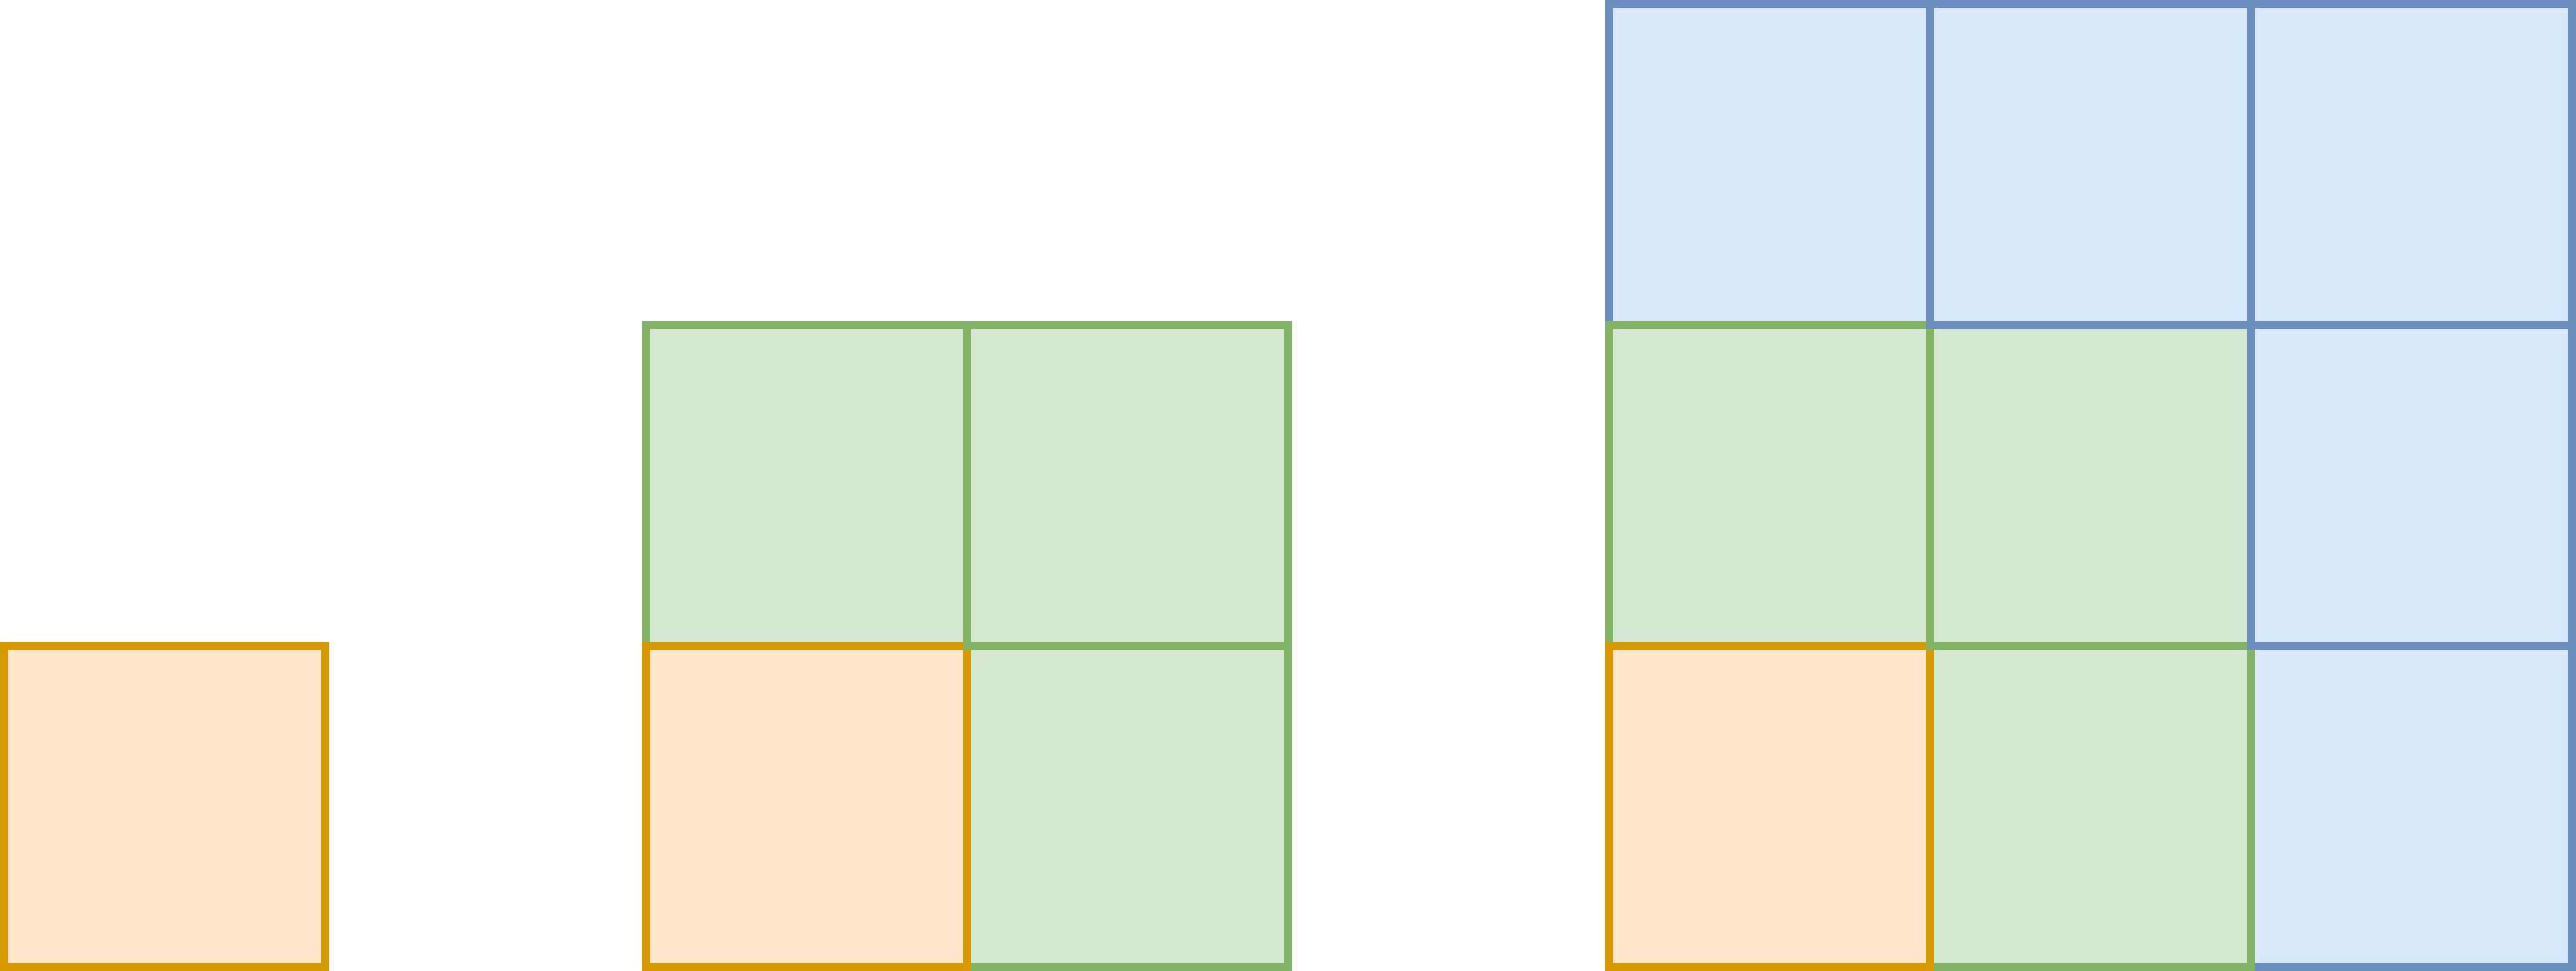
\includegraphics[width=0.5\textheight]{../figures/Summe.png}\qquad \dots
        %\caption{Idee}
        %
    \end{figure}
\end{frame}

\begin{frame}[fragile]{Beispiel}
Zeigen Sie $\displaystyle\sum_{i = 0}^{n} (2i+1) = (n+1)^2,\quad\forall n \in\mathbb{N}$.
\begin{alertblock}{Induktionsanfang IA}
    Zeige Aussage gilt für $n\defeq0$:\\
    \begin{align*}
        \sum_{i = 0}^{0} (2i+1) &\overset{!}{=} (0+1)^2\\
        \iff 2 * 0 + 1 &\overset{!}{=}1^2\\
        \iff 1 &= 1 \qquad\checkmark
    \end{align*}
\end{alertblock}
\end{frame}

\begin{frame}[fragile]{Beispiel}
Zeigen Sie $\displaystyle\sum_{i = 0}^{n} (2i+1) = (n+1)^2,\quad\forall n \in\mathbb{N}$.
\begin{alertblock}{Induktionsanfang IA}
    Aussage gilt für $n\defeq0$, da $\sum_{i = 0}^{0} (2i+1) = (0+1)^2$
\end{alertblock}
\begin{alertblock}{Induktionsvorraussetzung IV}
    Ang. Aussage gilt für $n \in\mathbb{N}$.
\end{alertblock}
\begin{alertblock}{Induktionsschritt IS}
    Zeige Aussage gilt für alle n+1 unter Nutzung der I.V.:\\
    $\sum_{i = 0}^{\alert{n+1}} (2i+1) \overset{!}{=} (\alert{(n+1)}+1)^2$
\end{alertblock}
\end{frame}

\begin{frame}[fragile]{Beispiel}
\small\begin{alertblock}{Induktionsschritt}
    Zeige Aussage gilt für alle n+1 unter Nutzung der I.V.:
    \begin{align*}
        \onslide<1->{&\sum_{i = 0}^{n+1} (2i+1)&\overset{!}{=} ((n+1)+1)^2}\\
        \onslide<2->{\iff&\sum_{i = 0}^{\alert<2>{n}} (2i+1) + \sum_{i = \alert<2>{n+1}}^{n+1} (2i+1)&\overset{!}{=} (n+2)^2}\\
        \onslide<3->{\iff&\sum_{i = 0}^{n} (2i+1) + ( 2(n+1)+1 )&\overset{!}{=} n^2 + 2 * 2n + 2^2}\\
        \onslide<4->{\overset{\alert<4>{IV}}\iff&\alert<4>{(n+1)^2} + ( 2(n+1)+1 )&\overset{!}{=} n^2+4n+4}\\
        \onslide<5->{\iff&n^2+2n+1^2+2n+2+1&\overset{!}{=} n^2+4n+4}\\
        \onslide<6>{\iff&n^2+4n+4&\alert<6>{=} n^2+4n+4}
    \end{align*}
\end{alertblock}
\end{frame}

\begin{frame}[fragile]{Beispiel}
Zeigen Sie $\displaystyle\sum_{i = 0}^{n} (2i+1) = (n+1)^2,\quad\forall n \in\mathbb{N}$.
\begin{alertblock}{Induktionsanfang IA}
    Aussage gilt für $n\defeq0$, da $\sum_{i = 0}^{0} (2i+1) = 1^2$
\end{alertblock}
\begin{alertblock}{Induktionsvorraussetzung IV}
    Ang. Aussage gilt für ein (beliebiges aber festes) $n \in\mathbb{N}$.
\end{alertblock}
\begin{alertblock}{Induktionsschritt IS}
    Aussage gilt für alle n+1 unter Nutzung der I.V., da\\
    $\sum_{i = 0}^{n+1} (2i+1) = ((n+1)+1)^2$
\end{alertblock}
\alert{$\leadsto$ Aussage gilt für alle n.}\qed
\end{frame}


{\setbeamercolor{palette primary}{bg=ExColor}
\begin{frame}[fragile]{Denkpause}
    \begin{alertblock}{Aufgaben}
    Versuche dich an den folgenden Induktionsbeweisen.
    \end{alertblock}

    \metroset{block=fill}
    \begin{block}{Normal}
        $\displaystyle\sum_{i=0}^{n} i = \frac{n(n+1)}{2}$, für alle $n \in \mathbb{N}$
    \end{block}
    \begin{block}{Schwerer}
        $\displaystyle\prod_{i=1}^{n} 4^i = 2^{n(n+1)}$, für alle $n \in \mathbb{N}\setminus \{0\}$
    \end{block}
\end{frame}
}

%\subsubsection{Lösungen normal}
{\setbeamercolor{palette primary}{bg=ExColor}
\begin{frame}<handout:0>[fragile]{Lösungen: normale Aufgabe}
    Zu zeigen: $\displaystyle\sum_{i=0}^{n} i = \frac{n(n+1)}{2}$ gilt für alle $n \in \mathbb{N}$.
    \begin{alertblock}{Induktionsanfang IA}
        Aussage gilt für $n\defeq 0$, da $\displaystyle\sum_{i=0}^{0} i = 0 = \frac{0(0+1)}{2}$.
    \end{alertblock}
    \begin{alertblock}{Induktionsvorraussetzung IV}
        Ang. Aussage gilt für $n \in\mathbb{N}$.
    \end{alertblock}
    \begin{alertblock}{Induktionsschritt IS}
        Zeige Aussage gilt für alle $n+1$ unter Nutzung der I.V.:\\
        $\displaystyle\sum_{i=0}^{\alert{n+1}} i \overset{!}{=} \frac{(\alert{n+1})((\alert{n+1})+1)}{2}$
    \end{alertblock}
\end{frame}


\begin{frame}<handout:0>[fragile]{Lösungen: normale Aufgabe}
\small\begin{alertblock}{Induktionsschritt}
    Zeige Aussage gilt für $n+1$ unter Nutzung der I.V.:
    \begin{align*}
        \onslide<1->{&\displaystyle\sum_{i=0}^{\alert<1>{n+1}} i &\overset{!}{=} \frac{(\alert<1>{n+1})((\alert<1>{n+1})+1)}{2}}\\
        \onslide<2->{\iff&(\displaystyle\sum_{i=0}^{n} i)+(n+1) &\overset{!}{=} \frac{(n+1)(n+2)}{2}}\\
        \onslide<3->{\iff&(\displaystyle\sum_{i=0}^{n} i)+(n+1) &\overset{!}{=} \frac{n^2+3n+2}{2}}\\
        \onslide<4->{\overset{\alert<4>{IV}}\iff&\alert<4>{\frac{n(n+1)}{2}}+(n+1) &\overset{!}{=} \frac{n^2+3n+2}{2}}\\
        \onslide<5->{\iff&\frac{n^2+n}{2}+\frac{2n+2}{2} &\overset{!}{=} \frac{n^2+3n+2}{2}}\\
        \onslide<6->{\iff&\frac{n^2+3n+2}{2} &\alert{=} \frac{n^2+3n+2}{2}}\\
    \end{align*}
\end{alertblock}
\end{frame}


\begin{frame}<handout:0>[fragile]{Lösungen: normale Aufgabe}
    Zu zeigen: $\displaystyle\sum_{i=0}^{n} i = \frac{n(n+1)}{2}$ gilt für alle $n \in \mathbb{N}$.
    \begin{alertblock}{Induktionsanfang IA}
        Aussage gilt für $n\defeq 0$, da $\displaystyle\sum_{i=0}^{0} i = 0 = \frac{0(0+1)}{2}$.
    \end{alertblock}
    \begin{alertblock}{Induktionsvorraussetzung IV}
        Ang. Aussage gilt für $n \in\mathbb{N}$.
    \end{alertblock}
    \begin{alertblock}{Induktionsschritt IS}
        Zeige Aussage gilt für $n+1$ unter Nutzung der I.V.:\\
        $\displaystyle\sum_{i=0}^{\alert{n+1}} i \overset{!}{=} \frac{(\alert{n+1})((\alert{n+1})+1)}{2}$ gilt für alle $n \in \mathbb{N}$
    \end{alertblock}
    \alert{$\leadsto$ Aussage gilt für alle $n$.}\qed
\end{frame}
}

% \begin{frame}[standout]
%   Fragen dazu?
% \end{frame}

%\subsubsection{Lösungen schwerer}
{\setbeamercolor{palette primary}{bg=ExColor}
\begin{frame}<handout:0>[fragile]{Lösungen: schwerere Aufgabe}
    Zu zeigen: $\displaystyle\prod_{i=1}^{n} 4^i = 2^{n(n+1)}$, für alle $n \in \mathbb{N}\setminus \{0\}$.
    \begin{alertblock}{Induktionsanfang IA}
        Aussage gilt für $n\defeq 1$, da $\displaystyle\prod_{i=1}^{1} 4^i = 4^1 = 4 = 2^2 = 2^{1(1+1)}$.
    \end{alertblock}
    \begin{alertblock}{Induktionsvorraussetzung IV}
        Ang. Aussage gilt für $n \in\mathbb{N}\setminus \{0\}$.
    \end{alertblock}
    \begin{alertblock}{Induktionsschritt IS}
        Zeige Aussage gilt für $n+1$ unter Nutzung der I.V.:\\
        $\displaystyle\prod_{i=1}^{\alert{n+1}} 4^i \overset{!}{=} 2^{(\alert{n+1})((\alert{n+1})+1)}$
    \end{alertblock}
\end{frame}

\begin{frame}<handout:0>[fragile]{Lösungen: schwerere Aufgabe}
\small\begin{alertblock}{Induktionsschritt}
    Zeige Aussage gilt für $n+1$ unter Nutzung der I.V.:
    \begin{align*}
        \onslide<1->{&\displaystyle\prod_{i=1}^{\alert<1>{n+1}} 4^i &\overset{!}{=} 2^{(\alert<1>{n+1})((\alert<1>{n+1})+1)}}\\
        \onslide<2->{\iff&(\displaystyle\prod_{i=1}^{n} 4^i) * 4^{(n+1)} &\overset{!}{=} 2^{(n+1)(n+2)}}\\
        \onslide<3->{\overset{\alert<3>{IV}}\iff&\alert<3>{(2^{n(n+1)})} * 4^{(n+1)} &\overset{!}{=} 2^{n^2+3n+2}}\\
        \onslide<4->{\iff&2^{n^2+n} * 2^{2(n+1)} &\overset{!}{=} 2^{n^2+3n+2}}\\
        \onslide<5->{\iff&2^{n^2+n} * 2^{2n+2} &\overset{!}{=} 2^{n^2+3n+2}}\\
        \onslide<6->{\iff&2^{(n^2+n)+(2n+2)} &\overset{!}{=} 2^{n^2+3n+2}}\\
        \onslide<7->{\iff&2^{n^2+3n+2} &\alert{=} 2^{n^2+3n+2}}
    \end{align*}
\end{alertblock}
\end{frame}


\begin{frame}<handout:0>[fragile]{Lösungen: schwerere Aufgabe}
     Zu zeigen: $\displaystyle\prod_{i=1}^{n} 4^i = 2^{n(n+1)}$, für alle $n \in \mathbb{N}\setminus \{0\}$.
    \begin{alertblock}{Induktionsanfang IA}
        Aussage gilt für $n\defeq 1$, da $\displaystyle\prod_{i=1}^{1} 4^i = 4^1 = 4 = 2^2 = 2^{1(1+1)}$.
    \end{alertblock}
    \begin{alertblock}{Induktionsvorraussetzung IV}
        Ang. Aussage gilt für $n \in\mathbb{N}\setminus \{0\}$.
    \end{alertblock}
    \begin{alertblock}{Induktionsschritt IS}
        Zeige Aussage gilt für $n+1$ unter Nutzung der I.V.:\\
        $\displaystyle\prod_{i=1}^{\alert{n+1}} 4^i \overset{!}{=} 2^{(\alert{n+1})((\alert{n+1})+1)}$ gilt für alle $n \in \mathbb{N}\setminus \{0\}$
    \end{alertblock}
    \alert{$\leadsto$ Aussage gilt für alle $n$.}\qed
\end{frame}
}

% \begin{frame}[standout]
%   Fragen dazu?
% \end{frame}
